\documentclass{article}
\usepackage{amsmath}
\usepackage{amssymb}
\usepackage{graphicx}

\title{CSE3504 Homework}
\author{Isaac Piegat}
\date{11/19/2024}

\begin{document}

\maketitle

\section*{Problem 1:}
\begin{enumerate}
    \item[(a)] 

    The expected waiting time for $n = 3$ arrivals is:
    \[
    \mathbb{E}[T_3] = \frac{n}{\lambda} = \frac{3}{0.1} = 30 \, \text{minutes}
    \]

    Thus, the expected waiting time is 30 minutes. \newline
    
    \item[(b)] 

    The probability that fewer than 3 patients arrive in the first 60 minutes is:
    
    \[
    P(N(60) < 3) = P(N(60) = 0) + P(N(60) = 1) + P(N(60) = 2)
    \]
    
    Using the Poisson probability formula:
    \[
    P(N(t) = k) = \frac{e^{-\lambda t} (\lambda t)^k}{k!}
    \]
    with $\lambda = 0.1$ and $t = 60$, we compute:
    \[
    P(N(60) = 0) = e^{-6}, \quad P(N(60) = 1) = 6e^{-6}, \quad P(N(60) = 2) = 18e^{-6}
    \]
    
    Adding these:
    \[
    P(N(60) < 3) = e^{-6} + 6e^{-6} + 18e^{-6} = 25e^{-6}
    \]
    
    Evaluating numerically in R:
    \begin{verbatim}
    lambda <- 0.1
    t <- 60
    prob <- exp(-lambda * t) * (1 + lambda * t + (lambda * t)^2 / 2)
    prob
    \end{verbatim}
    
    The result is approximately:
    \[
    P(N(60) < 3) \approx 0.002478
    \]
    
    Thus, the probability is approximately 0.25\%.
\end{enumerate}

\section*{Problem 2:}

\begin{enumerate}
    \item[(a)]
    \[
    P = 
    \begin{bmatrix}
    0 & 0.75 & 0.2 & 0.05 \\
    0.05 & 0.2 & 0 & 0.45 \\
    0 & 0.4 & 0.3 & 0.2 \\
    0 & 0.15 & 0.3 & 0.55
    \end{bmatrix}
    \]
    \item[(b)] 

\[
P(\text{Average} \to \text{Poor}) = 0.00
\]

Thus, the probability is $0.00$.

\item[(c)] 

\[
P(\text{Rich} \to \text{Poor in 3 years}) = (P^3)_{1,3}
\]

Using R to calculate $P^3$:

\begin{verbatim}
P <- matrix(c(0, 0.75, 0.2, 0.05,
              0.05, 0.2, 0, 0.45,
              0, 0.4, 0.3, 0.2,
              0, 0.15, 0.3, 0.55), nrow=4, byrow=TRUE)

P3 <- P %*% P %*% P
prob <- P3[1, 3]
prob
\end{verbatim}

The result is:
\[
P(\text{Rich} \to \text{Poor in 3 years}) \approx 0.174
\]

Thus, the probability is 0.174.

\item[(d)]

$\pi = [\pi_{\text{Rich}}, \pi_{\text{Average}}, \pi_{\text{Poor}}, \pi_{\text{In Debt}}]$ are:

\[
\pi \cdot P = \pi
\]

Expanded, these equations are:

\[
\pi_{\text{Rich}} = 0.75\pi_{\text{Rich}} + 0.05\pi_{\text{Average}}
\]
\[
\pi_{\text{Average}} = 0.2\pi_{\text{Rich}} + 0.2\pi_{\text{Average}} + 0.4\pi_{\text{Poor}} + 0.15\pi_{\text{In Debt}}
\]
\[
\pi_{\text{Poor}} = 0.2\pi_{\text{Rich}} + 0.3\pi_{\text{Poor}} + 0.3\pi_{\text{In Debt}}
\]
\[
\pi_{\text{In Debt}} = 0.05\pi_{\text{Rich}} + 0.45\pi_{\text{Average}} + 0.2\pi_{\text{Poor}} + 0.55\pi_{\text{In Debt}}
\]

The normalization condition is:
\[
\pi_{\text{Rich}} + \pi_{\text{Average}} + \pi_{\text{Poor}} + \pi_{\text{In Debt}} = 1
\]

\item[(e)]


Using R:

\begin{verbatim}
P <- matrix(c(0, 0.75, 0.2, 0.05,
              0.05, 0.2, 0, 0.45,
              0, 0.4, 0.3, 0.2,
              0, 0.15, 0.3, 0.55), nrow=4, byrow=TRUE)

P_steady <- P %^% 100
steady_state <- P_steady[1, ]
steady_state
\end{verbatim}

The result is:
\[
\pi = [\pi_{\text{Rich}}, \pi_{\text{Average}}, \pi_{\text{Poor}}, \pi_{\text{In Debt}}] \approx [0.052, 0.313, 0.375, 0.260]
\]

Thus, the steady-state probabilities are:
\[
\pi_{\text{Rich}} \approx 0.052, \quad \pi_{\text{Average}} \approx 0.313, \quad \pi_{\text{Poor}} \approx 0.375, \quad \pi_{\text{In Debt}} \approx 0.260
\]

\item[(f)]

\textbf{R Code:}

\begin{verbatim}
# Install and load igraph
install.packages("igraph")
library(igraph)

nodes <- c("Rich", "Average", "Poor", "In Debt")
edges <- c(
  "Rich", "Average", "Rich", "Poor", "Rich", "In Debt",
  "Average", "Rich", "Average", "Average", "Average", "In Debt",
  "Poor", "Average", "Poor", "Poor", "Poor", "In Debt",
  "In Debt", "Average", "In Debt", "Poor", "In Debt", "In Debt"
)
weights <- c(0.75, 0.2, 0.05, 0.05, 0.2, 0.45, 0.4, 0.3, 0.2, 0.15, 0.3, 0.55)

g <- graph(edges = edges, directed = TRUE)
E(g)$weight <- weights  # Assign weights to edges

plot(
  g,
  vertex.label = nodes,
  edge.label = round(E(g)$weight, 2),
  layout = layout.circle,
  edge.arrow.size = 0.5,
  main = "State Transition Diagram"
)
\end{verbatim}

Result below: 
\begin{center}
    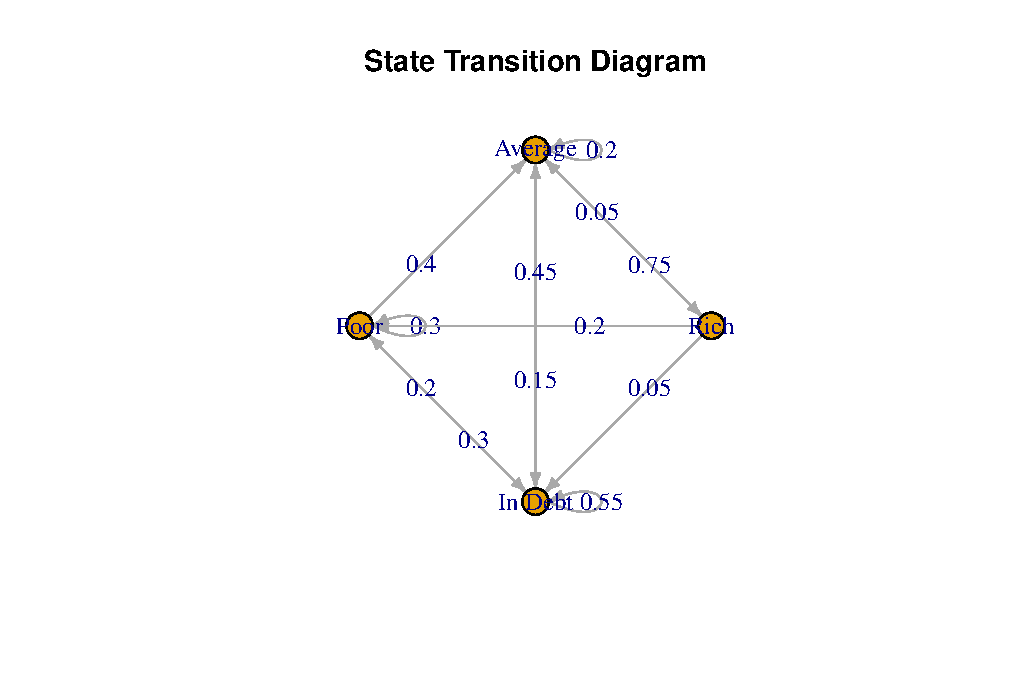
\includegraphics[width=0.8\textwidth]{HW5_Prob2_Partf.pdf}
\end{center}

\section*{Problem 3:}
\item[(a)]

\[
X \sim \text{Binomial}(n = 5, p = 0.85)
\]

The probability of acceptable attendance is:
\[
P(X \geq 4) = P(X = 4) + P(X = 5)
\]

Using the binomial probability formula:
\[
P(X = k) = \binom{n}{k} p^k (1-p)^{n-k}
\]

Compute each term:
\[
P(X = 4) = \binom{5}{4} (0.85)^4 (0.15)^1
\]
\[
P(X = 5) = \binom{5}{5} (0.85)^5 (0.15)^0
\]

Add the probabilities:
\[
P(X \geq 4) = P(X = 4) + P(X = 5)
\]

Using R:

\begin{verbatim}
# R Code
n <- 5
p <- 0.85
prob <- dbinom(4, size = n, prob = p) + dbinom(5, size = n, prob = p)
prob
\end{verbatim}

Thus, the probability that a student has acceptable attendance is approximately:
\[
P(X \geq 4) \approx 0.754
\]

    \item[(b)]

\[
Y \sim \text{Binomial}(n = 200, p = 0.754)
\]

The mean and variance of $Y$ are:
\[
\mu = np = 200 \cdot 0.754 = 150.8, \quad \sigma^2 = np(1-p) = 200 \cdot 0.754 \cdot (1 - 0.754) = 36.9688
\]

Approximating $Y$ as a Normal distribution:
\[
Y \approx \mathcal{N}(\mu = 150.8, \sigma = \sqrt{36.9688} \approx 6.08)
\]

We compute:
\[
P(Y \geq 170) = P\left(Z \geq \frac{170 - 150.8}{6.08}\right)
\]

The z-score is:
\[
Z = \frac{170 - 150.8}{6.08} \approx 3.15
\]

Using the standard normal distribution table:
\[
P(Z \geq 3.15) \approx 0.0008
\]

In R:

\begin{verbatim}
# R Code
n <- 200
p <- 0.754
mu <- n * p
sigma <- sqrt(n * p * (1 - p))
prob <- 1

\end{verbatim}

\item[(c)]

\[
\mathbb{E}[Y] = n \cdot p
\]

Substituting the values $n = 200$ and $p = 0.754$:
\[
\mathbb{E}[Y] = 200 \cdot 0.754 = 150.8
\]

Thus, the expected number of students with acceptable attendance is:
\[
\mathbb{E}[Y] = 150.8
\]

\end{enumerate}

\section*{Problem 4:}
\begin{enumerate}

\item[(a)]

\[
P = 
\begin{bmatrix}
1 & 0 & 0 & 0 & 0 \\
\frac{24}{25} & \frac{1}{25} & 0 & 0 & 0 \\
0 & \frac{47}{50} & \frac{3}{50} & 0 & 0 \\
0 & 0 & \frac{47}{50} & \frac{3}{50} & 0 \\
0 & 0 & 0 & \frac{24}{25} & \frac{1}{25}
\end{bmatrix}
\]

\[
Q = 
\begin{bmatrix}
\frac{24}{25} & \frac{1}{25} & 0 & 0 \\
0 & \frac{47}{50} & \frac{3}{50} & 0 \\
0 & 0 & \frac{47}{50} & \frac{3}{50} \\
\end{bmatrix}
\]

The fundamental matrix $N$ is:
\[
N = (I - Q)^{-1}
\]

Sum rows of $N$ for result in R:

\begin{verbatim}
# R Code
library(MASS)

Q <- matrix(c(24/25, 1/25, 0, 0,
              0, 47/50, 3/50, 0,
              0, 0, 47/50, 3/50), nrow=3, byrow=TRUE)

I <- diag(nrow(Q)) 
N <- solve(I - Q) 

expected_time <- rowSums(N)
expected_time
\end{verbatim}

The result is:
\[
\text{Expected time to absorption} \approx [1.04, 1.98, 3.93]
\]

Thus, the expected number of interactions before absorption for each transient state is approximately \(1.04\), \(1.98\), and \(3.93\).

\item[(b)]

\textbf{R Code:}

\begin{verbatim}
# Install and load igraph
install.packages("igraph")
library(igraph)

nodes <- c("1 Heard (Absorbing)", "2 Heard", "3 Heard", "4 Heard", "5 Heard (Absorbing)")
edges <- c(
  2, 1,  # 2 Heard -> 1 Heard (Absorbing)
  2, 3,  # 2 Heard -> 3 Heard
  3, 2,  # 3 Heard -> 2 Heard
  3, 4,  # 3 Heard -> 4 Heard
  4, 3,  # 4 Heard -> 3 Heard
  4, 5   # 4 Heard -> 5 Heard (Absorbing)
)
weights <- c(1/25, 24/25, 3/50, 47/50, 3/50, 47/50)

g <- make_graph(edges = edges, directed = TRUE)
E(g)$weight <- weights  # Assign weights to edges

V(g)$name <- nodes

plot(
  g,
  vertex.label = V(g)$name,
  edge.label = round(E(g)$weight, 2),
  layout = layout.circle,
  edge.arrow.size = 0.5,
  main = "State Transition Diagram for Rumor Spread"
)
\end{verbatim}

Diagram:
\begin{center}
    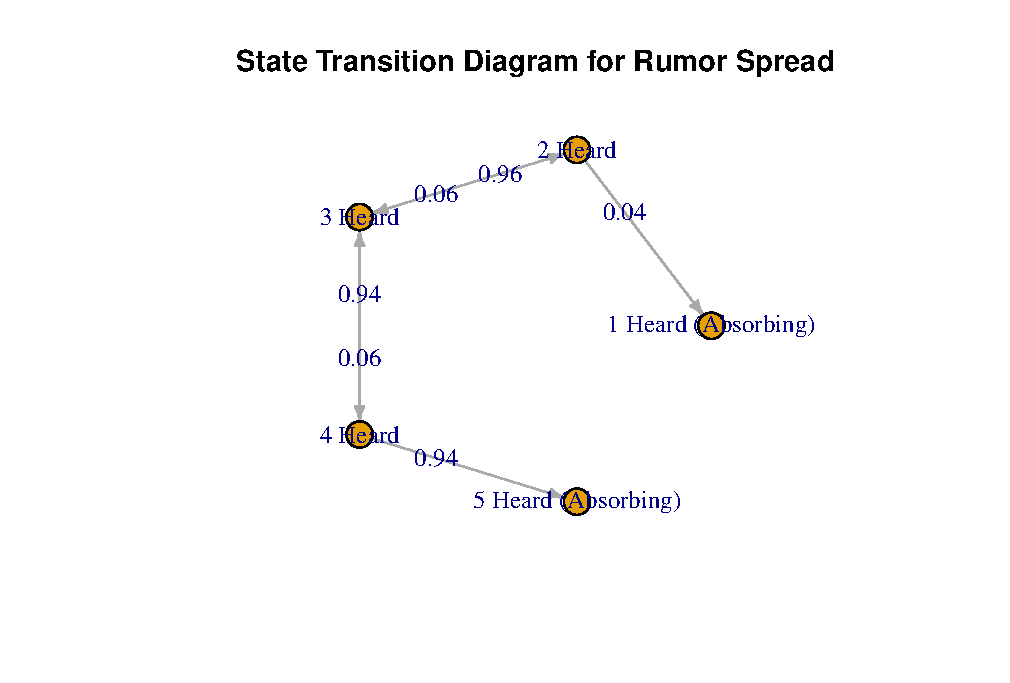
\includegraphics[width=0.8\textwidth]{HW5_Prob4_Partb.pdf}
\end{center}

\end{enumerate}
\end{document}